\documentclass[justified,nofonts,nobib]{tufte-book}
% Use tufte-book, not tufte-handout as the documentclass
% use pdfLatex as the compiler
\pdfoutput=1
\usepackage[utf8]{inputenc}
\usepackage[english]{babel}
\usepackage{biblatex}
\addbibresource{references.bib}
\usepackage{csquotes}

\usepackage{siunitx}
\DeclareSIUnit\torr{Torr}
\usepackage{amssymb}
\usepackage{wasysym}
\usepackage{listings}
\usepackage{soul}
\usepackage{graphicx}

% Customize the sections:
\usepackage{titlesec}
% Turn on section numbering
\setcounter{secnumdepth}{2}
% chapter format
\titleformat{\chapter}%
  {\huge\sffamily\bfseries}% format applied to label+text
  {\llap{\colorbox{cyan}{\parbox{1.5cm}{\hfill\itshape\huge\color{white}\thechapter}}}}% label
  {2pt}% horizontal separation between label and title body
  {}% before the title body
  []% after the title body
% section format
\titleformat{\section}%
  {\sffamily\Large\bfseries}% format applied to label+text
  {\thesection}% label
  {1 em}% horizontal separation between label and title body
  {}% before the title body
  []% after the title body
  
\titleformat{\subsection}%
  {\sffamily\large}% format applied to label+text
  {\thesubsection}% label
  {4 pt}% horizontal separation between label and title body
  {}% before the title body
  []% after the title body
  
\usepackage{hyperref}
\hypersetup{
    colorlinks=true,
    linkcolor=cyan,
    filecolor=magenta,
    pdftitle={Thesis Ehud Behar}
}

%%% Document %%%
\begin{document}
	\chapter{Abstract}\label{chap:abstract}
	\chapter{Introduction}\label{chap:intro}
	An introduction to LWFA, our experiment, etc.
	\chapter{Theoretical background}\label{chap:background}
	A background to the plasma state of matter, including a definition of plasma, characteristics and important equations used in this research, and a background to plasma spectroscopy.
	\section{Definition of plasma}
Plasma is an "ionized" gas in which at least one of the electrons in an atom has been stripped free, leaving a positively charged nucleus (ion). The resulting charged ions and electrons are not bound - but approximately neutral on a macroscopic scale. To maintain this state of matter, a large amount of energy is required, with the aim of dissociating molecules and ionizing atoms, and to give ions and electrons enough kinetic energy to avoid immediate recombination. Therefore it is an unbalanced state of matter which requires, for its maintenance, a permanent supply of energy. On earth, plasma usually exists only in a vacuum; Otherwise, air will cool the plasma so that the ions and electrons will recombine into normal neutral atoms. It is important to be aware that a plasma cannot be treated simply as an ordinary gas which is electrically conducting. Due to the long range of the inter-particle forces each charged particle in a plasma interacts with a large number of other charged particles resulting in \emph{collective behaviour}. Plasma oscillations and Debye screening are typical examples of this collective behaviour.
\section{Concept of Temperature}
It is customary in plasma physics to describe temperatures in units of energy, since $T$ and $\left<E\right>$ are so closely related. To avoid confusion on the number of dimensions involved, it is not $\left<E\right>$ but the energy corresponding to $k_B T$ that is used to denote the temperature. For example, by a \SI{2}{\electronvolt} plasma we mean that $k_B T = \SI{1}{\electronvolt}$.

The familiar Maxwell-Boltzmann distribution corresponds to a system of particles that have reached thermodynamic equilibrium and uniform distributions of density and temperature. In plasma diagnostics, the assumption of full thermodynamic equilibrium has to be relaxed. In what follows we will assume that in a small neighbourhood (element of volume) of any point in the system, there is an equilibrium situation described by a local Maxwell-Boltzmann distribution function. For larger spatial scales there may exist gradients of $T$ but these scales are so large that locally the equilibrium is not perturbed; time variation of $T$ may exist, but on such slow time scale that instantaneous equilibrium is a very good approximation. This approximation is  called \emph{local thermodynamic equilibrium} (LTE). The assumption of LTE is a very powerful one, since it allows us to use the familiar results of statistical mechanics and thermodynamics. The relative populations of different states of an atom or ion are described by the Boltzmann equation:
\begin{equation}
		\frac{n_i}{n_j}=\frac{g_i}{g_j}e^{\frac{E_i-E_j}{k_B T}}=\frac{g_i}{g_j}e^{-\frac{h\nu_{ij}}{k_B T}}
\end{equation}
where $g_{i,j}$ are the degeneracies of the states. 

\section{Saha Equation}\label{sec:saha}
For a system in LTE, the Saha equation gives the amount of ionization to be expected in a gas, as a function of temperature and the concentration of electrons:
\begin{equation}
		\frac{n_i}{n_n}= \left(\frac{2 \pi m_e k_B T}{h^2}\right)^{3/2}\frac{T^{3/2}}{n_i}e^{-U_i/k_B T} \approx \SI{2.4e21}{\per \metre\cubed \per\kelvin\tothe{3/2}} \frac{T^{3/2}}{n_i}e^{-U_i/k_B T}
\end{equation}
By combining the Boltzmann equation and Saha equation, we can determine the population for any particular atomic state, and thus predict the strength of the emission line produced by the plasma.
\section{Plasma Oscillation}\label{sec:oscillation}
The transfer of electrons from a given region of space to a neighbouring region induces a charge separation. This local charge gives rise to an electric field $E$. Since the electrons are much lighter than the ions, they respond much more rapidly to the electric field, and the motion of the ions can be neglected in first instance. The electric field pulls the electrons back to their initial position in order to reduce the local charge separation which is the source of the electric field. Those electrons produce another non-equilibrium distribution in the opposite direction, and so on, performing an oscillatory motion \sidenote{Eq. \ref{eq:index_of_refraction} for $\omega_p$ does not depend on $k$, so the group velocity $\mathrm{d}\omega / \mathrm{d}k$ is zero - the disturbance does not propagate.}, with the Coulomb force acting as the restoring force and the mass of the electron as the inertia. This is called a plasma oscillation, defined as
\begin{equation}
		\omega_p=\sqrt{\frac{n_e e^2}{m_e \varepsilon_0}}\si[per-mode=fraction]{\radian\per\sec}.\label{eq:plasma-frequency}
\end{equation}
For a typical plasma density of $n_e \sim \SI{e18}{\per\cubic\cm}$, we get $\omega_p=\SI{5.6e13}{\radian\per\sec}$, which lies in the microwave range.

\section{Debye shielding length}\label{sec:debye}
The Debye length determines the effective interaction between charged particles in a plasma. The potential field $\phi$ around a charged particle is effectively screened by the cloud of the other charged particles; its force range is now confined within a certain characteristic length, $\lambda_D$, called the Debye shielding length, determined by the density and the temperature of the plasma:
\begin{equation}
\phi(r)=\frac{q_i}{4\pi\varepsilon_0 r}\exp{\left(-\frac{r}{\lambda_D}\right)},
\end{equation}
where
\begin{equation}
\lambda_D=\sqrt{\frac{\varepsilon_0 k_B T_e}{n_e e^2}}=\sqrt{\frac{k_B T}{m_e}}\frac{1}{\omega_p}.
\end{equation}
For a plasma with characteristic thermal energy of \SI{1}{\electronvolt}, number density $n_e \sim \SI{e18}{\per\cubic\cm}$, we get $\lambda_D \sim \SI{7}{\nm}$.
For any volume with a length scale $L$ satisfying 
\begin{equation}
L \ll \lambda_D,
\end{equation}
overall quasi-neutrality is a good approximation. This inequality is the first criterion for the definition of a plasma. If the dimension $L$ is near or less than $\lambda_D$, then our approximations break down and significant deviations from quasi-neutrality occur.
\section{The spectrum of Hydrogen and Stark Broadening}\label{sec:hydrogen}
The emission spectrum of atomic hydrogen, due to the electron making a transition between two energy levels, has been divided into a number of spectral series, with wavelengths given by the Rydberg formula. Transitions to the first excited state ($n_f=2$) are known to spectroscopists as the \textit{Balmer series} \sidenote{The others, to name a few, are Lyman ($n_f=1$) and Paschen ($n_f=3$).}, denoted historically as H\textsubscript{$\alpha$}, H\textsubscript{$\beta$}, H\textsubscript{$\gamma$} and so on, where H stands for the element Hydrogen. It is convenient to observe H\textsubscript{$\alpha$} ($n_i=3 \to n_f=2$, 656.23 nm) and H\textsubscript{$\beta$} ($n_i=4 \to n_f=2$ ,486.13 nm) because both fall in the visible region.

In addition to the familiar natural (lifetime) and Doppler broadening, in plasma spectroscopy an additional smearing of the lines is observed, named \textit{Stark Broadening} \sidenote{Classified under \textit{Pressure broadening} mechanism.}: When the density of charged particles in a plasma is sufficiently large, their electric micro-fields perturb the atomic energy levels\cite{Griem1974SpectralPlasmas.}; An emitting atom at a distance $r$ from an ion or electron is perturbed by an electric field $E=e/(4\pi \varepsilon_0 r^2)$, and the interaction between the atom and the field is described by the Stark effect. A perturbation proportional to $E$ exists only in the case of the hydrogen atom; for all other atoms the first non-vanishing interaction is the quadratic Stark effect\cite{Thorne1988Spectrophysics}, proportional to $E^2$ and thus to $1/r^4$.

Natural broadening smears out the H\textsubscript{$\alpha$} line by only 20 parts per billion, and Doppler broadening by 3 parts per million. Thus, in the presented measurements, we neglect these two, and focus solely on the Stark Broadening.

The line shape for the Stark broadening assumes that of a Lorentzian,
\begin{equation}
I\left( \lambda \right)=\frac{A^2}{4\left( \left(\lambda-\lambda_0\right)^2+\Delta \lambda_{1/2}^2\right)}. \label{eq:Stark_Broadening}
\end{equation}
where $\Delta \lambda_{1/2}\left[\si{\nm}\right]$ is the full width at half maximum for a profile centered at wavelength $\lambda_0$.

This phenomenon for hydrogen lines is very well understood, and the dependence of the line width on the plasma concentration and plasma density has been tabulated \cite{Griem1964PlasmaSpectroscopy,Griem1974SpectralPlasmas.}, but, from the theoretical point of view, there does not exist any model that enables accurate calculations of Stark broadening over a large electron density range\cite{Griem2000StarkPlasmas}. 

The following equation relates electron density to the width of the emission line for the H\textsubscript{alpha} line:
\begin{equation}
n_e=\left( \frac{\Delta\lambda_{1/2}}{\gamma\left(n_e,T_e\right)}\right)^{3/2}.
\end{equation}
$\gamma\left(n_e,T_e\right)$ may be evaluated numerically and experimentally\cite{Griem2005ComparisonResults}, the dependence of which on the plasma density and temperature is rather weak and it has been neglected in our measurements, at which the following was used:
\begin{equation}
n_e=\left( \frac{\Delta\lambda_{1/2}\text{[nm]}}{5.4}\right)^{3/2}. \label{eq:delta_lambda}
\end{equation}
\section{Index of refraction}\label{sec:indexrefraction}

The dispersion relation \cite{Chen1984IntroductionFusion} for an electromagnetic wave propagating in a plasma takes the form
\begin{equation}
\omega^2=\omega_p^2+c^2 k^2.
\end{equation}

Written as an expression for the index of refraction $\tilde{n}=c/v_\phi = ck/\omega$ (squared)\sidenote{Eq. \ref{eq:index_of_refraction} for $\omega^2\left( k \right)$ needs to be amended by multiplying the second term with a function of $\omega$, whether it is an ordinary (O) wave, an extra-ordinary (X) wave, or a circularly polarized (R or L) wave, according to the case. This doesn't change the fact that $\tilde{n}$ is still less that unity for each type of wave, thus not altering our present discussion.},
\begin{equation}
\tilde{n}^2=\frac{c^2 k^2}{\omega^2}=1-\frac{\omega_p^2}{\omega}, \label{eq:index_of_refraction}
\end{equation}

we see that the index of refraction is less than unity for a plasma, and it has some interesting consequences.

A convex plasma lens is divergent rather than convergent.
\textcolor{red}{Write about the radial density profile and cutoff frequency}
\begin{marginfigure}
    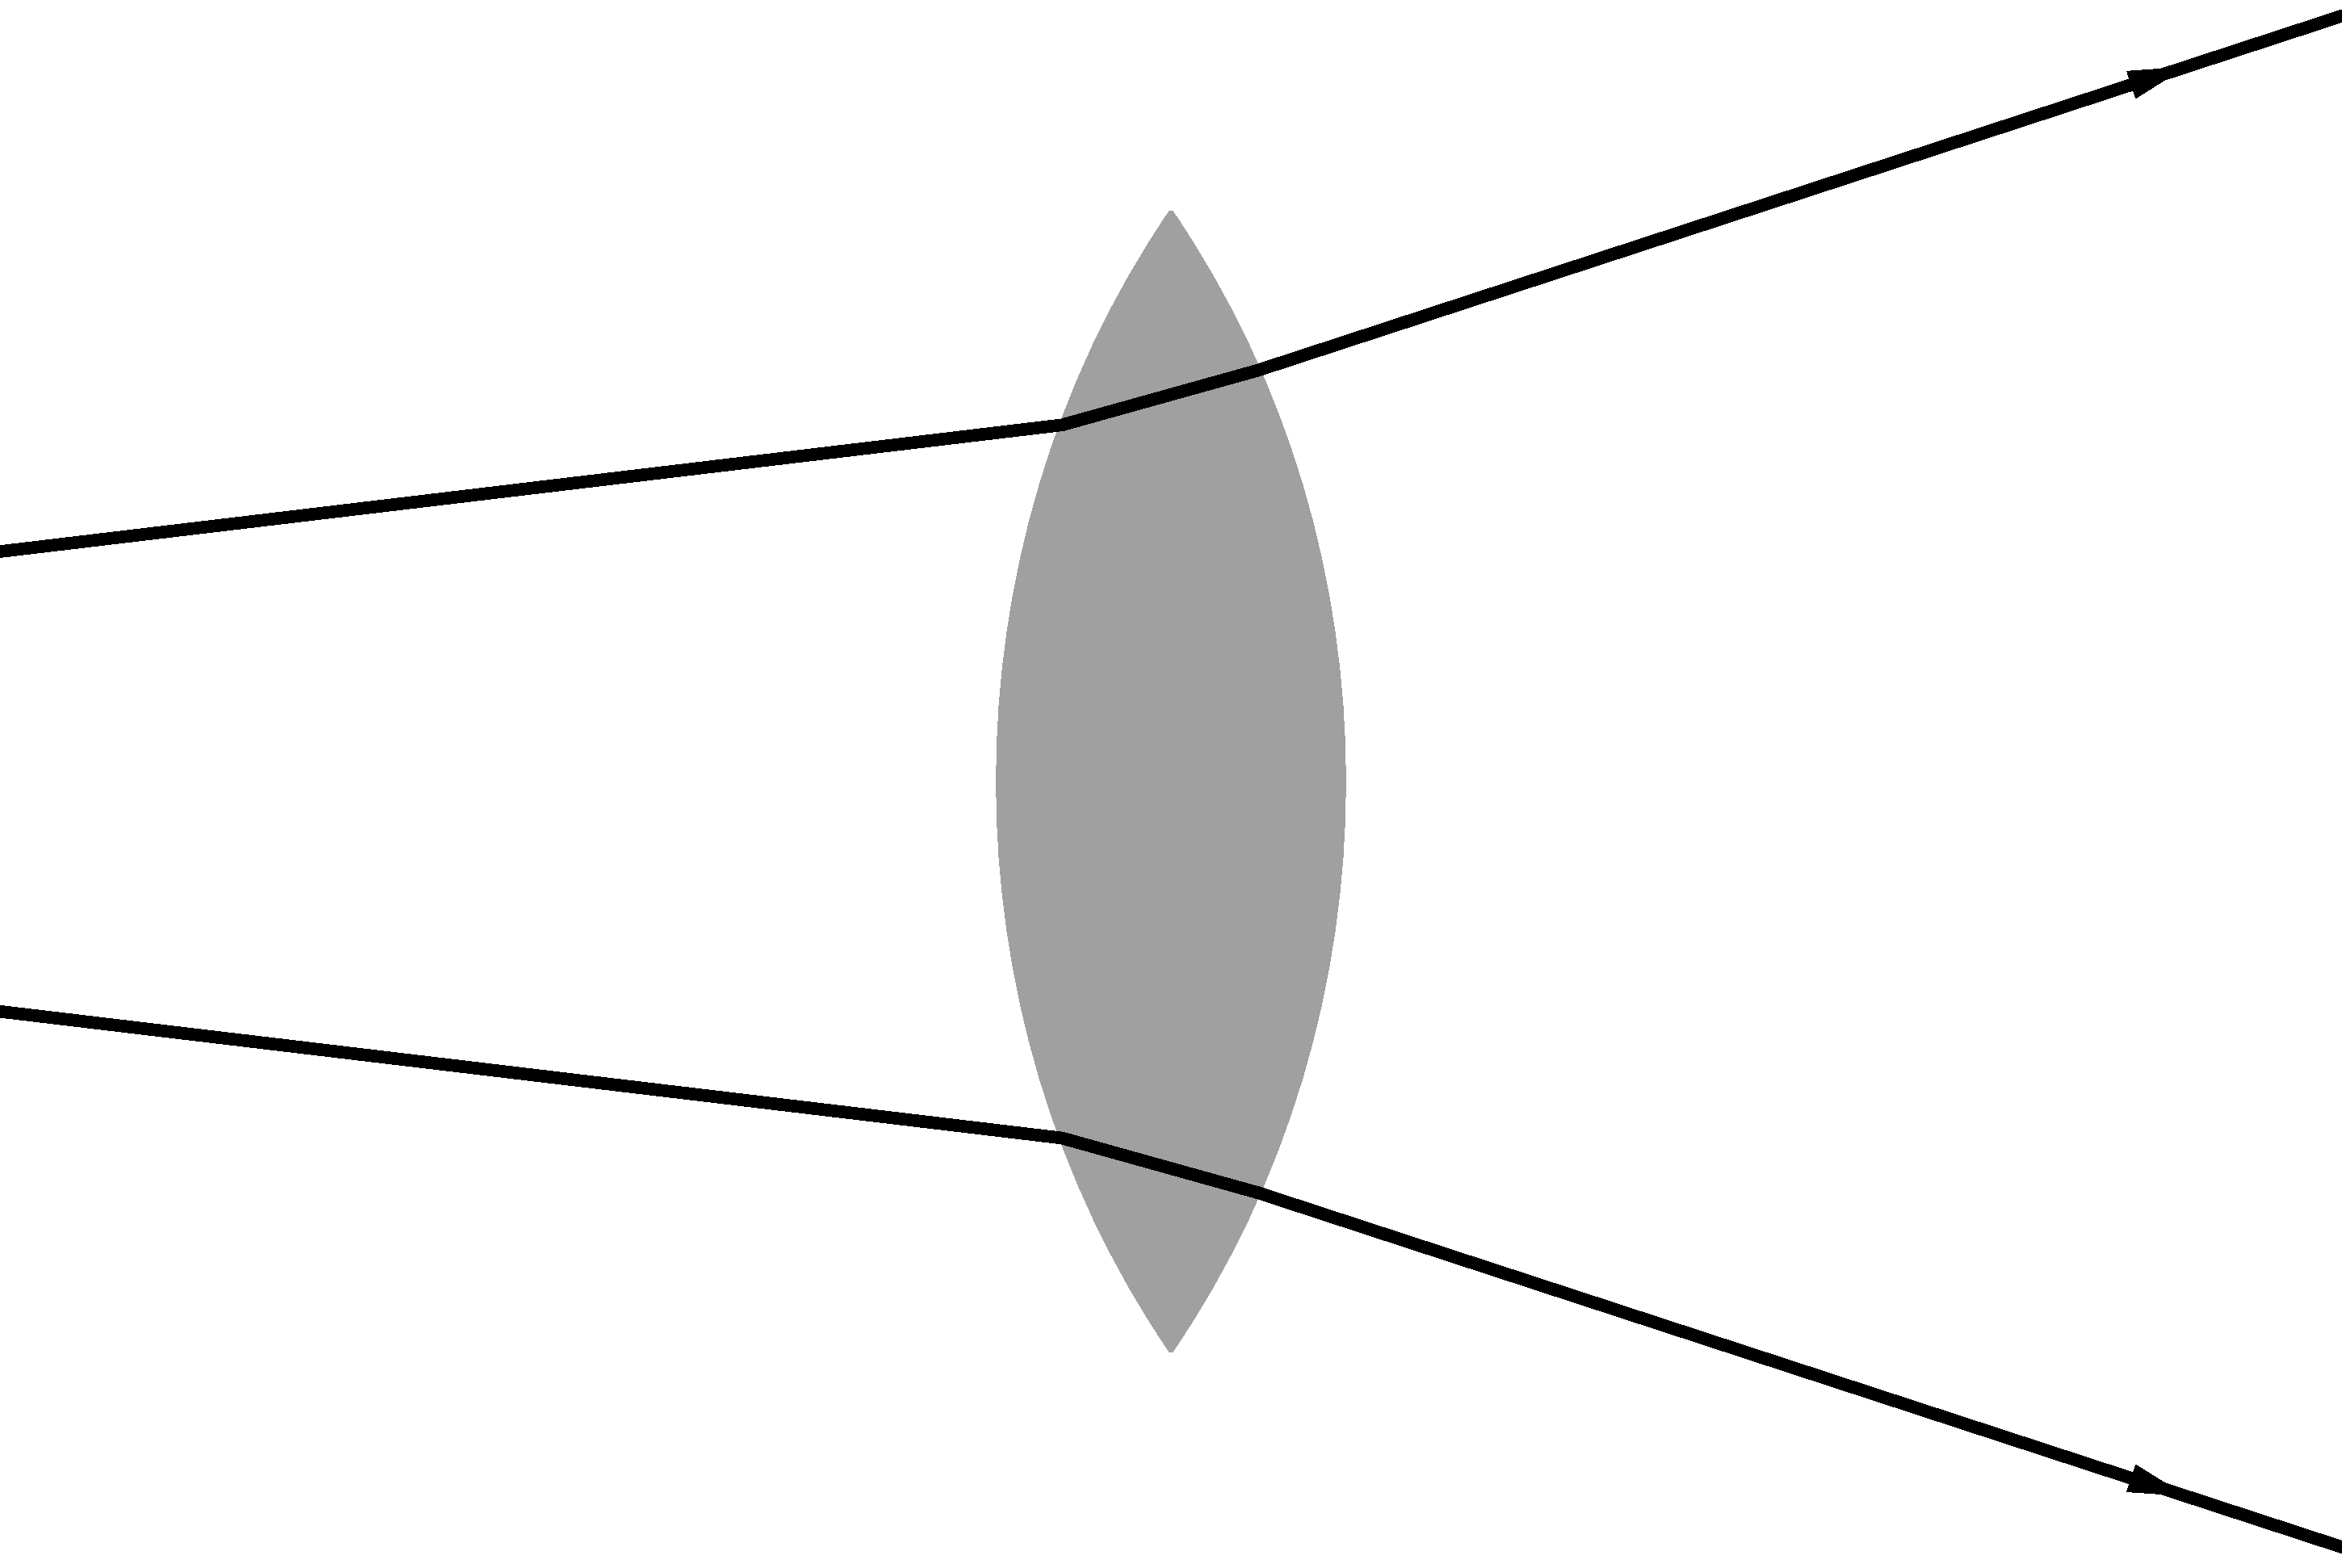
\includegraphics[width=\marginparwidth]{figures/chen4_30.pdf}
    \caption{A plasma lens has unusual optical properties, since the index of refraction is less than unity.}
    \label{fig:plasma_lens_chen}
\end{marginfigure}
For a \SI{800}{\nm} laser field transversing the plasma, \textcolor{red}{what happens}

\section{Wakefield and the acceleration of electrons in it}\label{sec:wakefield} 
Modern particle accelerators use radio-frequency (RF) waves travelling in metal cavities to accelerate particles. These waves have a longitudinal electric field which propagates near the speed of light allowing relativistic particles to remain in the accelerating phase of the field. Ionisation of the walls at high voltages means that they cannot support electric field gradients greater than $\sim 100$ \textcolor{blue}{write with siunitx} MVm\textsuperscript{-1}, though the operating limit is usually more like $\sim 10$ MVm\textsuperscript{-1}. This limits the highest energies achievable through cost, as each GeV of energy requires $\sim 100$ m of acceleration length.
If the limiting factor on the scale of the accelerator is ionisation of the material, then an attractive alternative, proposed by J. Dawson and T. Tajima\cite{Dawson1979} is to use a plasma as the medium for the acceleration mechanism, since a plasma can support arbitrarily high electric fields, limited only by the obtainable charge density \cite{Esarey2009PhysicsAccelerators}.

\textcolor{red}{Write correctly this paragraph; Get help from 2.3.1 in Antonio Giulietti}
A single laser pulse with a duration less than the plasma period excites a plasma wave via the action of the ponderomotive force. This force, caused by the laser intensity gradient, ejects all the electrons, leaving a bubble of the slow moving ions. This charge separation provides a large electric field. The ponderomotive force, related to the laser intensity gradient, is able to push electrons away from regions of high laser intensity, while the ions stay immobile because of their higher mass. As the pulse passes, the electrons are attracted back by the ion charge, forming a negative layer around the bubble and converging into an electron bunch behind the bubble.
Laser-driven plasma acceleration is a technique in which particles are accelerated by the field of an electron plasma wave (wakefield) trailing an intense laser pulse. Such large electric field generation can be achieved by focusing an ultra-short and powerful TW laser that provides a large electric field because of charge separation. Plasma formed by initiating a discharge in a narrow channel made within a tube (i.e., discharge capillary) satisfies promising
conditions for a plasma source to exploit LWFA. Since the middle of 1980s, Ultrashort laser pulses of sufficient energy have become possible and available, after the damage thershold inherent in optical amplifiers had been overcome by means of Chirped Pulse Amplification (CPA)\cite{Strickland1985CompressionPulses}.

To date, acceleration distances have been severely limited by the lack of a controllable method for extending the propagation distance of the focused laser pulse. In the absence of such guiding, the interaction length is at most of the order of the Rayleigh range. The problem of making a highly
focused laser pulse ($\sim 20 \mu$m) propagate over many tens of Rayleigh lengths without divergence can be solved by constructing a preformed plasma channel with a radial, continuous, ideally parabolic decrease of refraction index (see figure \textcolor{red}{figure rdp.svg}. Plasma waveguides of this type are formed dynamically, and their effectiveness
results from the corresponding increase of the plasma density.
\begin{marginfigure}
    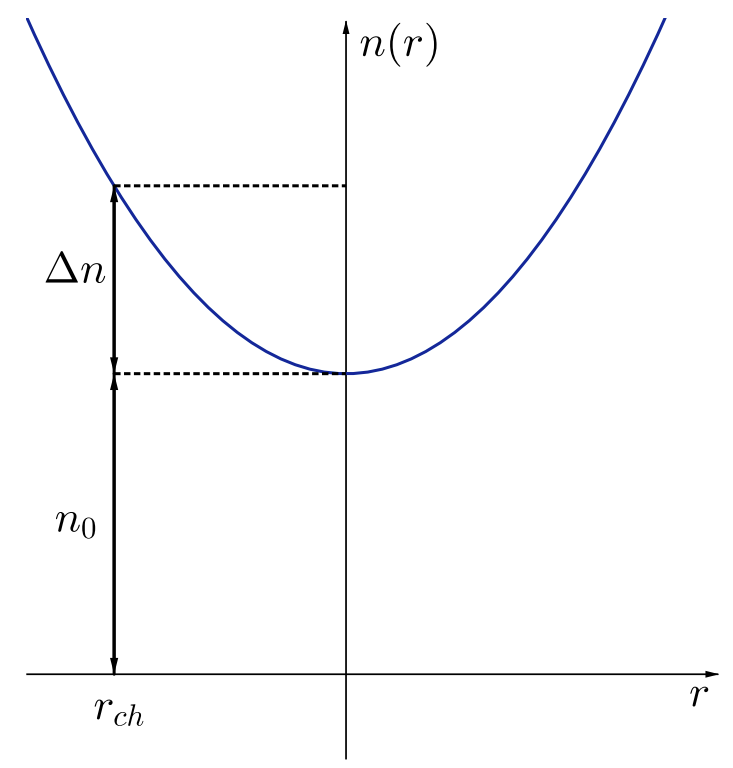
\includegraphics[width=\marginparwidth]{figures/rdp.PNG}
    \caption{Radial Density Profile (RDP)}
    \label{fig:rdp_parabola}
\end{marginfigure}
As stated in section \ref{sec:indexrefraction}, the refractive index of a plasma seen by an electromagnetic radiation with angular frequency $\omega$ (and corresponding wavelength $\lambda$) can be obtained from equation \ref{eq:index_of_refraction}:
\begin{equation} \label{eq:index_refraction_approx}
N_e(r)=N_e(0)+\Delta N_e\left( \frac{r}{r_m}\right)^2
\end{equation}
where
\begin{equation}
n_{cr}=\frac{\omega^2 \varepsilon_0 m}{e^2}=\frac{\pi}{\lambda^2 r_e} \label{eq:critical_density}
\end{equation}
is the critical plasma density, and $r_e$ is the classical electron radius. Equation \ref{eq:index_refraction_approx} thus shows explicitly that the refractive index peaks on the axis of a plasma channel if the density has there a minimum. 
The dependence $n(r)$ is usually termed the "radial density profile" (RDP). A parabolic RDP (figure \ref{fig:rdp_parabola}), given by equation \ref{eq:index_refraction_approx}, is of highly practical interest, because it is capable \cite{Sprangle1992PropagationPlasmas,Sprangle1992PropagationPlasmas} of guiding a tightly focused laser pulse while keeping its radius constant; It can help increase the dephasing length that will allow a longer propagation distance and a higher energy gain. 

\section{Paschen Curve}\label{sec:paschen}
Paschen's Law states that the breakdown voltage is a unique function of the product of gas pressure $p$ and the gap length $d$ for a particular gas. The curve is shown in figure \ref{fig:paschen_curve}.
\begin{marginfigure}
    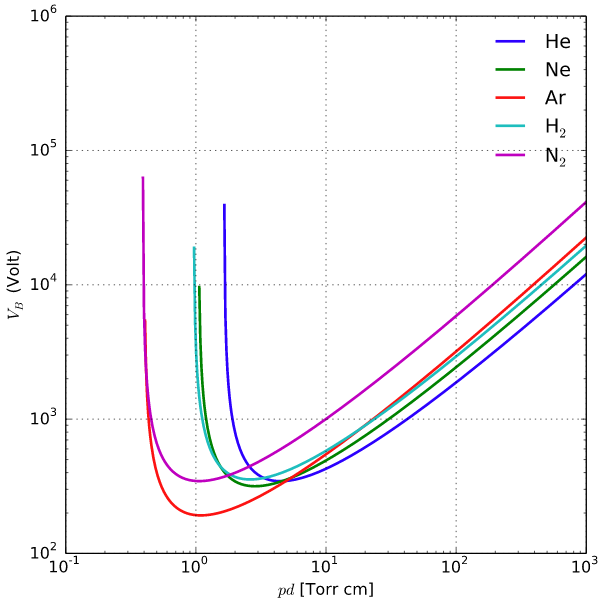
\includegraphics[width=\marginparwidth]{figures/paschen_curve.PNG}
    \label{fig:paschen_curve}
    \caption{Paschen curve --- voltage versus the pressure--gap length product.}
\end{marginfigure}

% \section{ccd,Spectrometer}\label{sec:ccd}

% \section{Diffraction grating}\label{sec:diffractiongrating}

\chapter{Thesis Goals}\label{chap:goals}
This thesis presents the results of the experimental study of various plasma processes in gas--filled capillary discharge.
\begin{enumerate}
  \item An experiment to lower and measure the jitter in igniting the plasma, generated in a mixture of N\textsubscript{2} and H\textsubscript{2} gas mixture, found to be in the scale of \SI{1}{\ns}, providing possibility for the synchronization with a high intensity laser or other auxiliary systems (f.e injectors).
  \item Gain for optical guiding of an \SI{84}{\MHz} oscillator laser passing through the capillary.
  \item Spectroscopy analysis on the plasma utilizing Stark broadening to convert the plasma's emission spectra to study its density and density profile; We confirmed the existence of a hollow density plasma profile and its density profile.
  \item \textcolor{red}{First experiment with a double capillary.}
\end{enumerate}
	\chapter{Methods}\label{chap:methods}

	\section{Experiment Scheme}\label{sec:experiment_scheme}
Our method of plasma generation is based on the laser trigger technique with the injection of N\textsubscript{2} and H\textsubscript{2} gas inside the capillary \cite{Bobrova2002SimulationsWaveguide,Spence2001InvestigationWaveguide}.
The waveguide is designed to operate in an evacuated chamber, maintained at $~$\SI{e-4}{\torr}.
\begin{figure}
\centering
    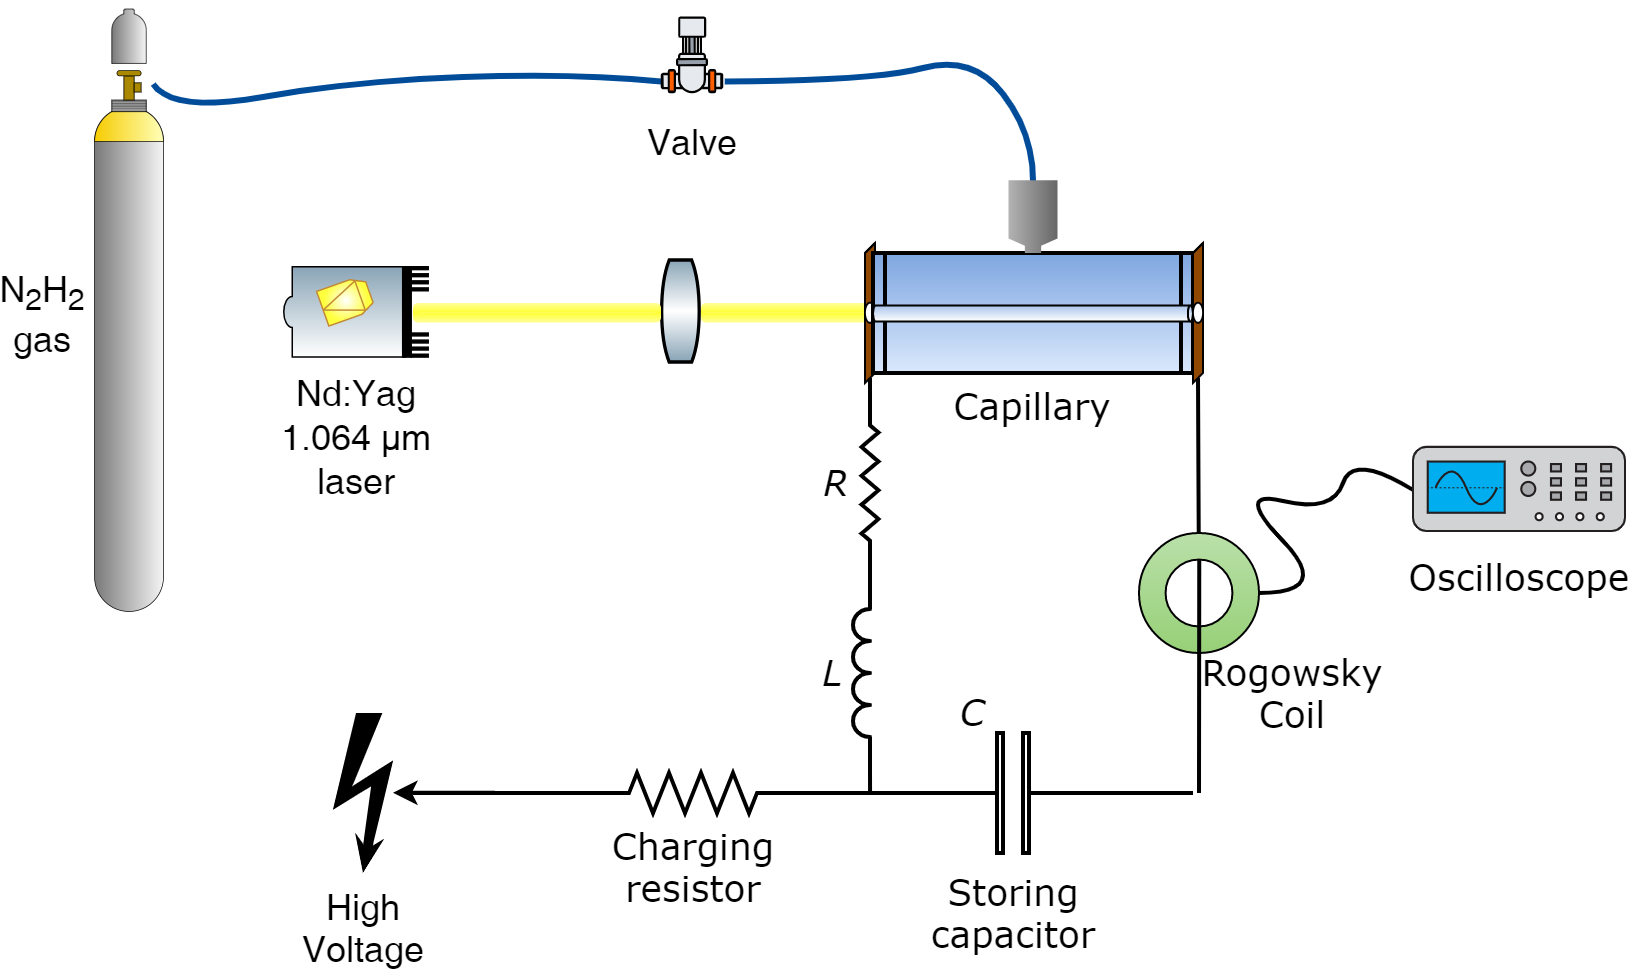
\includegraphics[width=\textwidth]{figures/Laser-based ignition scheme.png}
    \label{fig:scheme}
    \caption{Plasma generation in the N\textsubscript{2}+H\textsubscript{2} gas--filled capillary. The vacuum chamber has been omitted for clarity.}
    \end{figure}
The experimental system is shown in figure \ref{fig:scheme}, and applies to all forth--coming discussion,\textcolor{red}{except if I write about double capillary.}

Two electrodes are mounted at both ends of the capillary. Those electrodes are connected to a high-voltage source, which provides a pulse of a few kilovolts amplitude, during the opening of a valve \sidenote{Product of \textit{Parker Hannifin Corporation}, model 099-0340-900}, set to be opened for \SI{30}{\ms}, that fills the the capillary with gas. The ignition is achieved by the igniting laser pulse, that ionizes matter and detaches electrons \cite{Palchan2007ElectronChannel}, which in turn accelerate under the applied high voltage and in an avalanche manner, plasma discharge manifests inside the capillary. The created electron current effectively closes an electrical circuit, for which the plasma ignition acts as a switch. The discharge current is recorded by a Rogowski coil \sidenote{\textit{Pearson}, model 110A. A wide band current transformer with typical response time of less than \SI{50}{\ns}.} and the current profile is acquired by an oscilloscope.

	\section{Devices in use}\label{sec:devices}
The experiment was conducted using the following devices:
\begin{enumerate}
    \item Capillary
    \item Nd:Yag Laser, 1064 nm
    \item Oscillator laser, 800 nm
    \item High Voltage power supply
    \item Spectrograph and Andor ccd camera
    \item Photodiodes
    \item Optical Elements, viz., lenses and mirrors
    \item Rogowsky coil
    \item Digital delay and pulse generator board
    \item Gate valve
    \item Vacuum chamber
\end{enumerate}
\subsection{Capillary production}
The capillary is the medium at which the plasma channel forms. Its length is \SI{5}{\cm}, and its inner diameter is \SI{500}{\um}. The plastic unit is made of a photopolymer, created in a 3D printer. The capillary is shown in figure \ref{fig:capillaryCAD}. Note the circular extrusion in the upper face; The capillary is filled with gas from this inlet port.
\begin{figure}
    \centering
    \includegraphics{figures/capillaryCAD.png}
    \caption{}
    \label{fig:capillaryCAD}
\end{figure}
\subsection{Lasers used}\label{ssec:lasers}
In our system two laser were in use, igniting laser and \textcolor{red}{oscillator} laser:
\begin{itemize}
\item The first is \textit{Tempest 10}, a \SI{1.064}{\um} pulse laser, flashlamp pumped, Q-switched, Nd:Yag laser manufactured by \textit{New Wave Optics}. The pulse duration is $\tau \sim$ \SI{10}{\ns}, and with energy of up to $\sim$ \SI{200}{\mJ}. The ignition of the plasma is initiated by this laser pulse that ablates a small amount of surface in the inner wall of the capillary and produces seed ionization that triggers the discharge after $\sim$\SI{50}{\ns}. In the experiment the energy being used in most cases to obtain reliable ignition was \SIrange{50}{100}{\mJ}. \textcolor{red}{This is what I measured with a power meter. Ask Arie.} Misha said \href{https://aip.scitation.org/doi/full/10.1063/1.2149183}{here} \textcolor{red}{that it was 10 to 15 mJ and Ori pollak say it was 80 mJ.} The laser beam was delivered on the capillary axis through the negative electrode by a focusing lens (see Figure \textcolor{red}{figure number }), thus igniting the plasma. \st{This technique makes it possible to achieve very low shot-to-shot jitter of the ignition delay.}
\item The second laser is \textit{Mai Tai}, a \SI{800}{\nm} mode-locked oscillator, manufactured by \textit{Spectra Physics}, with a Ti:Sa crystal as the lasing medium.
\begin{marginfigure}
    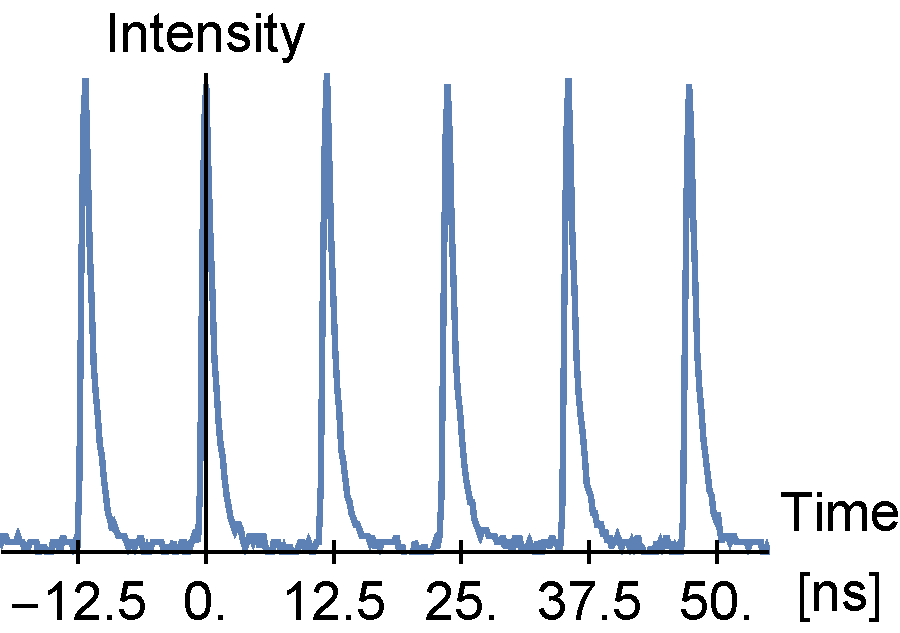
\includegraphics[width=\marginparwidth]{figures/oscillator/single.pdf}
    \label{fig:oscillator_single}
    \caption{Oscillator laser, \SI{84}{\MHz} temporal beam profile.}
\end{marginfigure}
It produces \SI{5}{\mJ} \textcolor{red}{check that}, \SI{20}{\fs} pulses at a \SI{84}{\MHz} rate. \textcolor{red}{I.e., a pulse every \SI{12.5}{\ns}.} This beam was directed through the capillary and recorded with a fast photo-diode (see figure \ref{fig:oscillator_single}), thus enabling one to compare the optical guiding at different times along the discharge process.
\end{itemize}
\subsection{High Voltage pulser}
\begin{marginfigure}
        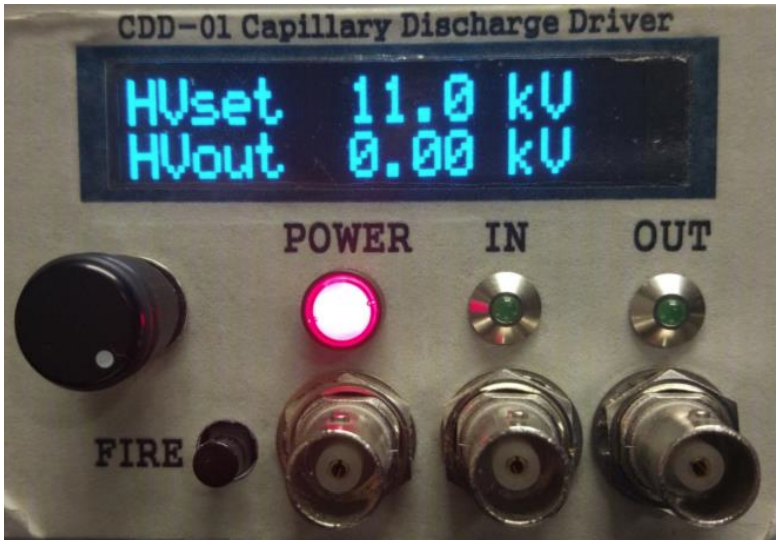
\includegraphics[width=\marginparwidth]{figures/hvpulser.PNG}
        \caption{Discharge Pulser high voltage, designed, built and Maintained by Michael Levin.}
\end{marginfigure}
The high voltage pulser provides the high voltage difference applied on the two electrodes. See picture on the right. Its key element is the energy storing capacitor that must be charged to a high voltage (that to be applied on the electrodes) and then discharged through the capillary and the rest of the electric chain. The pulser was designed, built, and still maintained, by Levin. See  \cite{Levin2009ExcitationAcceleration} pp. 46-47, for more information considering the setup and explanation of its operation.
	
\subsection{Spectrograph and Andor CCD camera}\label{ssec:spectro}
To measure the capillary plasma density and to validate the existence of a hollow radial density profile at the time segment optical guiding exist, we performed a direct spectroscopic study of the plasma emission. The plasma emission during the discharge was collected by an imaging system and imaged onto the entrance slit of a detection system, composed of a spectrometric instrument\sidenote{\textit{Spectra--Pro} model 300i}, fitted with a 2D 1024$\times$256 element intensified charge-coupled device (CCD) fast camera\sidenote{\textit{Andor}, model DH520.}. The CCD allows for recording images with both spectral and spatial resolution.

The detector gating and delay were set by a digital delay and pulse generator board\sidenote{\textit{Stanford Research Systems},\newline model DG--535.} that triggers the CCD camera.

\begin{figure}
\centering
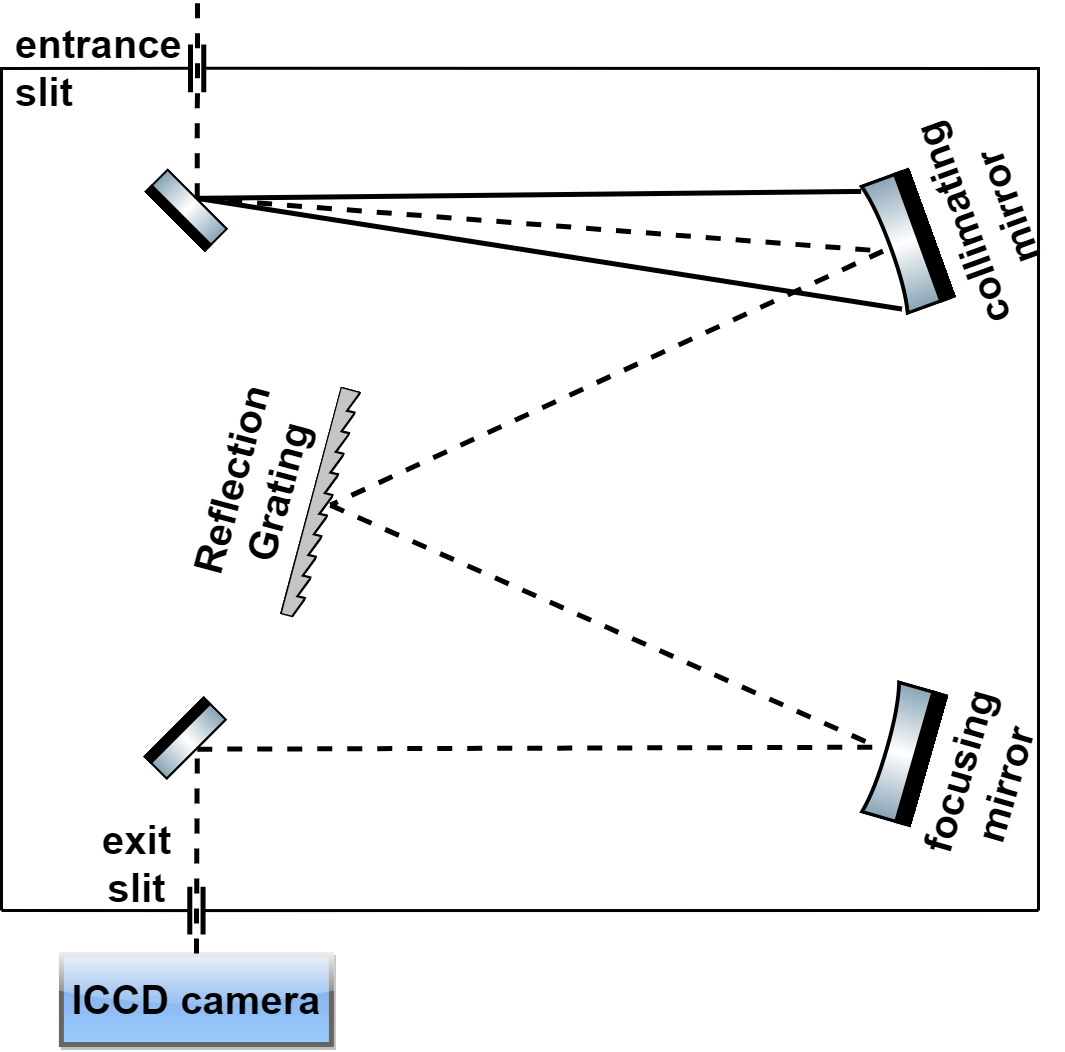
\includegraphics[width=\textwidth]{./figures/spectro/spectrometer.PNG}
\caption{Optical layout for the spectrometric instrument.}
\label{fig:spectrometer}
\end{figure}
The spectrometric instrument is a Czerny-Turner arrangement, made of a plane reflection grating. Light entering the entrance slit is collimated by a concave mirror and directed towards the plane reflection grating. Light diffracted from the grating forms a plane wave that is focused by another concave mirror onto the exit slit. Only one wavelength leaves the grating in the right direction to reach the exit slit, and tuning is achieved by rotating the grating, controlled by Andor's computer software. See figure \ref{fig:spectrometer}. In our measurements we used a 1800 lines/mm grating; Spatial resolution is controlled by the width of the entrance slit.

\subsection{Timings}
	\textcolor{red}{fill!}
	
\chapter{Experimental work}\label{chap:Experimental_work}
\section{Capillary discharge, Jitter}\label{sec:jitter}
Experiments in which plasma channels are supposed to be ready-to-use guiding media require a low ignition jitter (the spread in initiation of the current), so as to provide results reproducible on shot-to-shot basis. Typical guiding window lasts about \SIrange{50}{100}{\ns}, so ignition jitter of about \SI{10}{ns} would be tolerable.

This was our goal as a first experiment with the gas injected capillaries.

A schematically drawing of the system is shown in figure \ref{fig:scheme}.
\begin{marginfigure}
    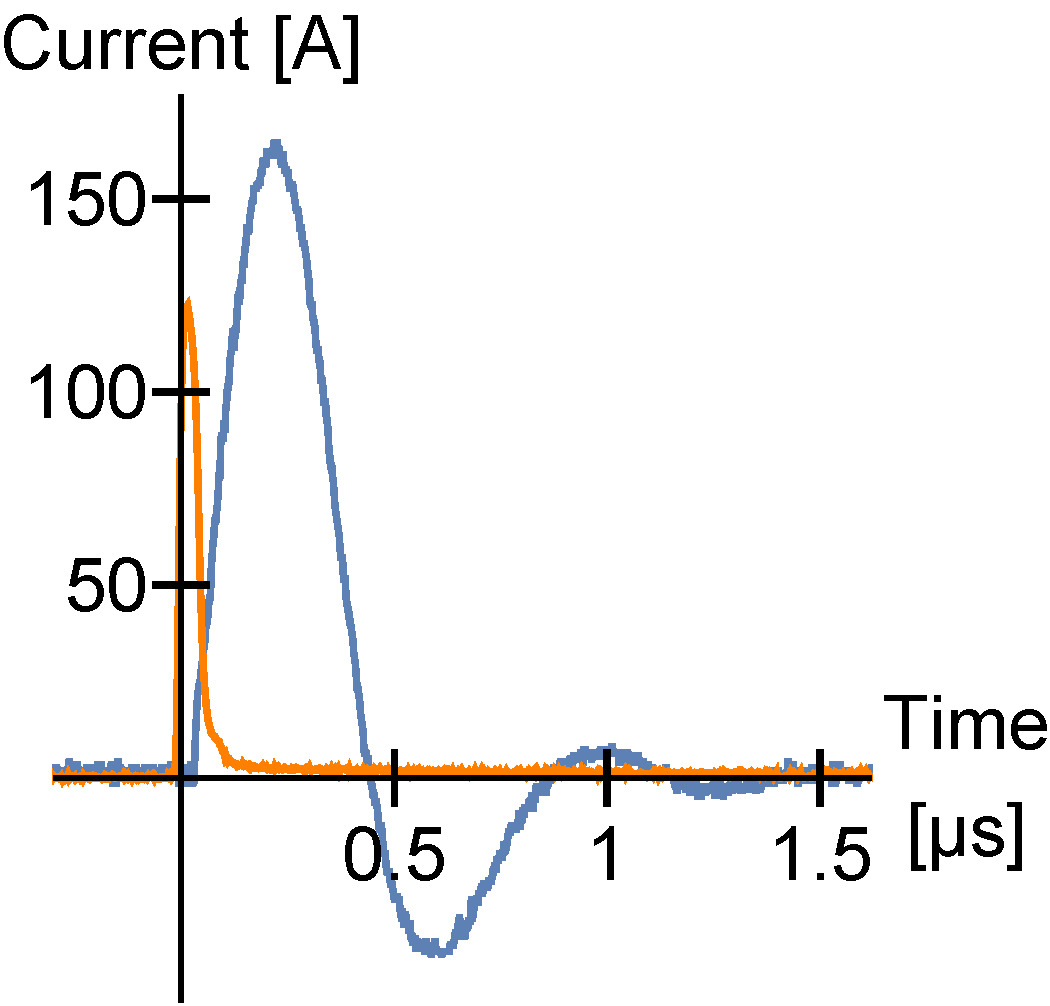
\includegraphics[width=\marginparwidth]{figures/jitter/discharge_sample.pdf}
    \caption{A typical discharge. Blue is current profile. Orange is photo--diode rise up from Nd:Yag. \textcolor{red}{Write more about it.}}
    \label{discharge_sample}
\end{marginfigure}
To anchor the discharge starting process to a fixed event to which we can refer, we mounted a photo--detector close to the igniting laser radiation output, thus enabling one to fix a time event at which the plasma discharge occurs; The photo--detector allows for visualizing the synchronization. Recording to an oscilloscope both the photo--diode rise-up signal and the current profile obtained from the Rogowsky coil, we monitored the igniting pulse and the discharge current for consecutive 50 ignitions performed at constant time intervals.
\begin{figure}
    \centering
    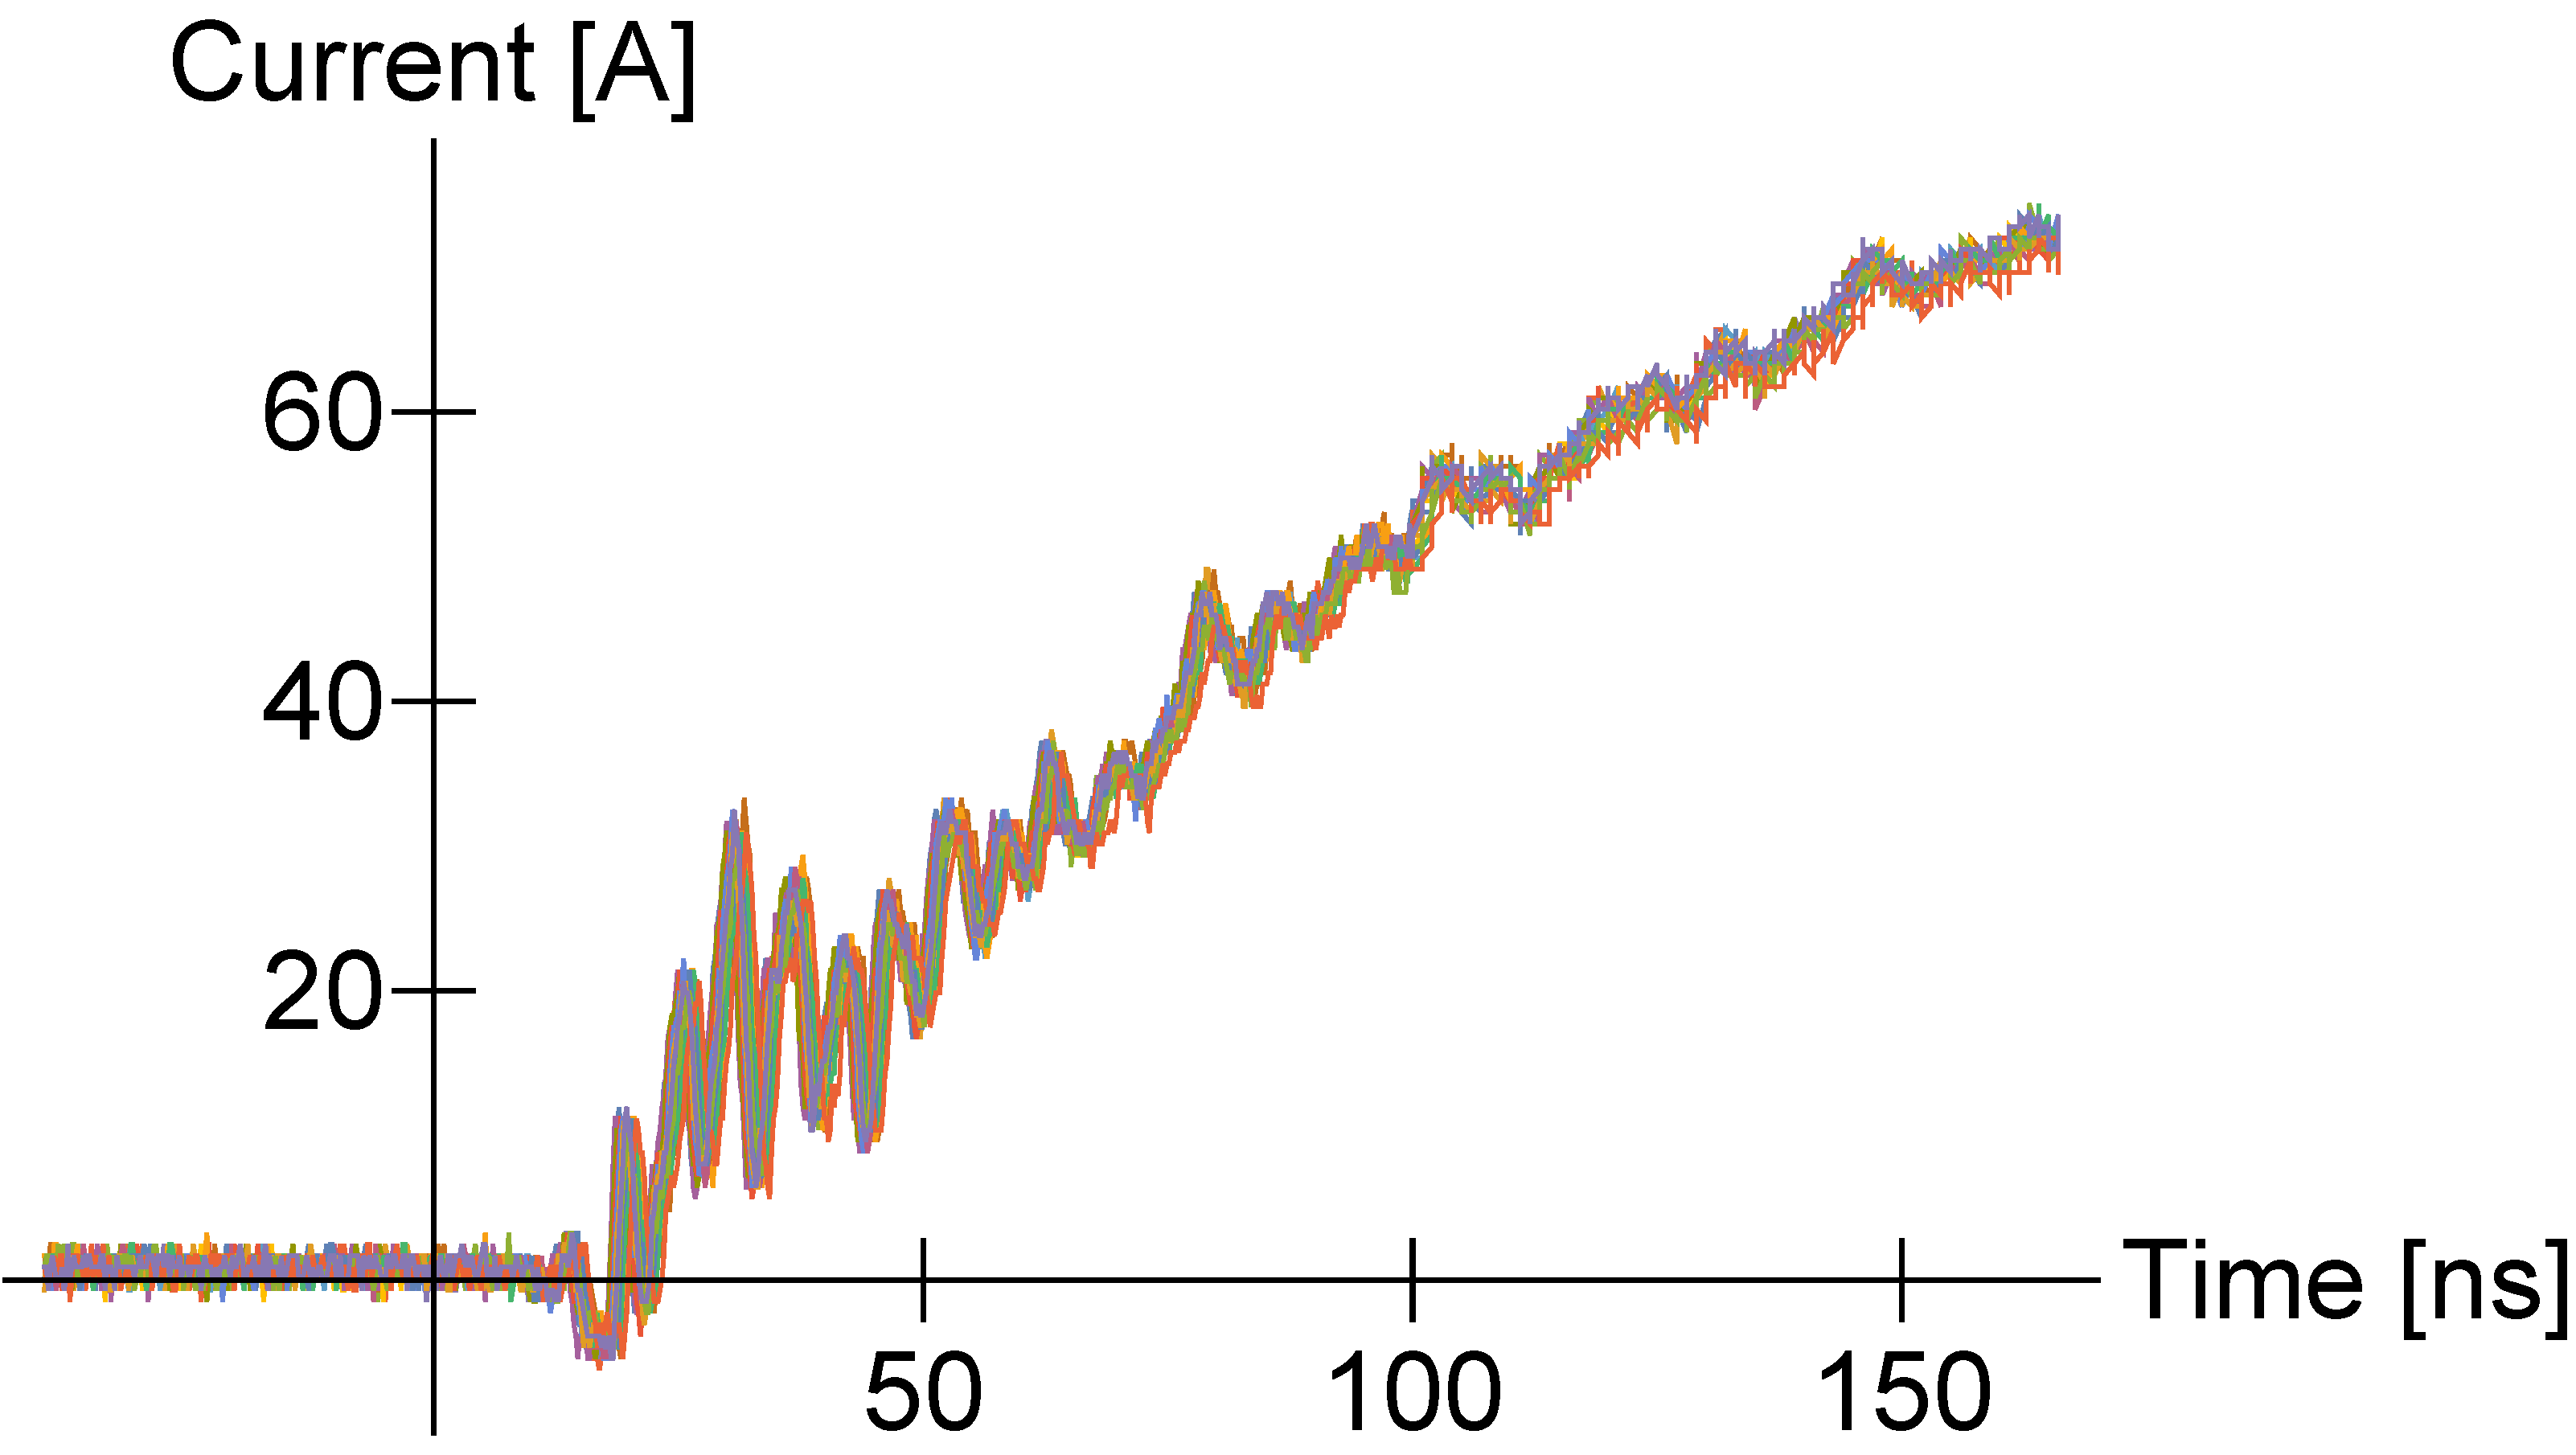
\includegraphics[width=\textwidth]{figures/jitter/low_jitter.pdf}
    \caption{Low jitter exhibiting \textcolor{red}{fix this.}}
    \label{fig:low_jitter}
\end{figure}

The time resolution is evaluated while taking into consideration both the oscilloscope sampling rate and the prior to ignition electrical components' jitter. The jitter is calculated as half the difference between the earliest and latest ignition timing of multiple independent ignitions. Overall, we evaluate the jitter to be
\begin{equation}
	\tau_\text{jitter}\approx 1\pm 0.36\si{\ns}
\end{equation}
This implies that we can determine the optical guiding timing of the incident laser to the plasma, with no concerns of shooting too early or too late with respect to the plasma channel. Also, we deduce that our system and its over all components is relatively stable and reliable.

On the contrary, a much less stable regime was observed if the experiment is repeated \textbf{without} the igniting laser pulse. The explanation is that the electrical breakdown evolves in a much less deterministic behaviour; The process of the electrons being ripped from the molecules in a cascading manner is rather not stable. The jitter observed under this constraint of absent igniting laser pulse is on the order of \SI{80}{\us}. See figure \ref{fig:multiple}.
\begin{figure}
    \centering
    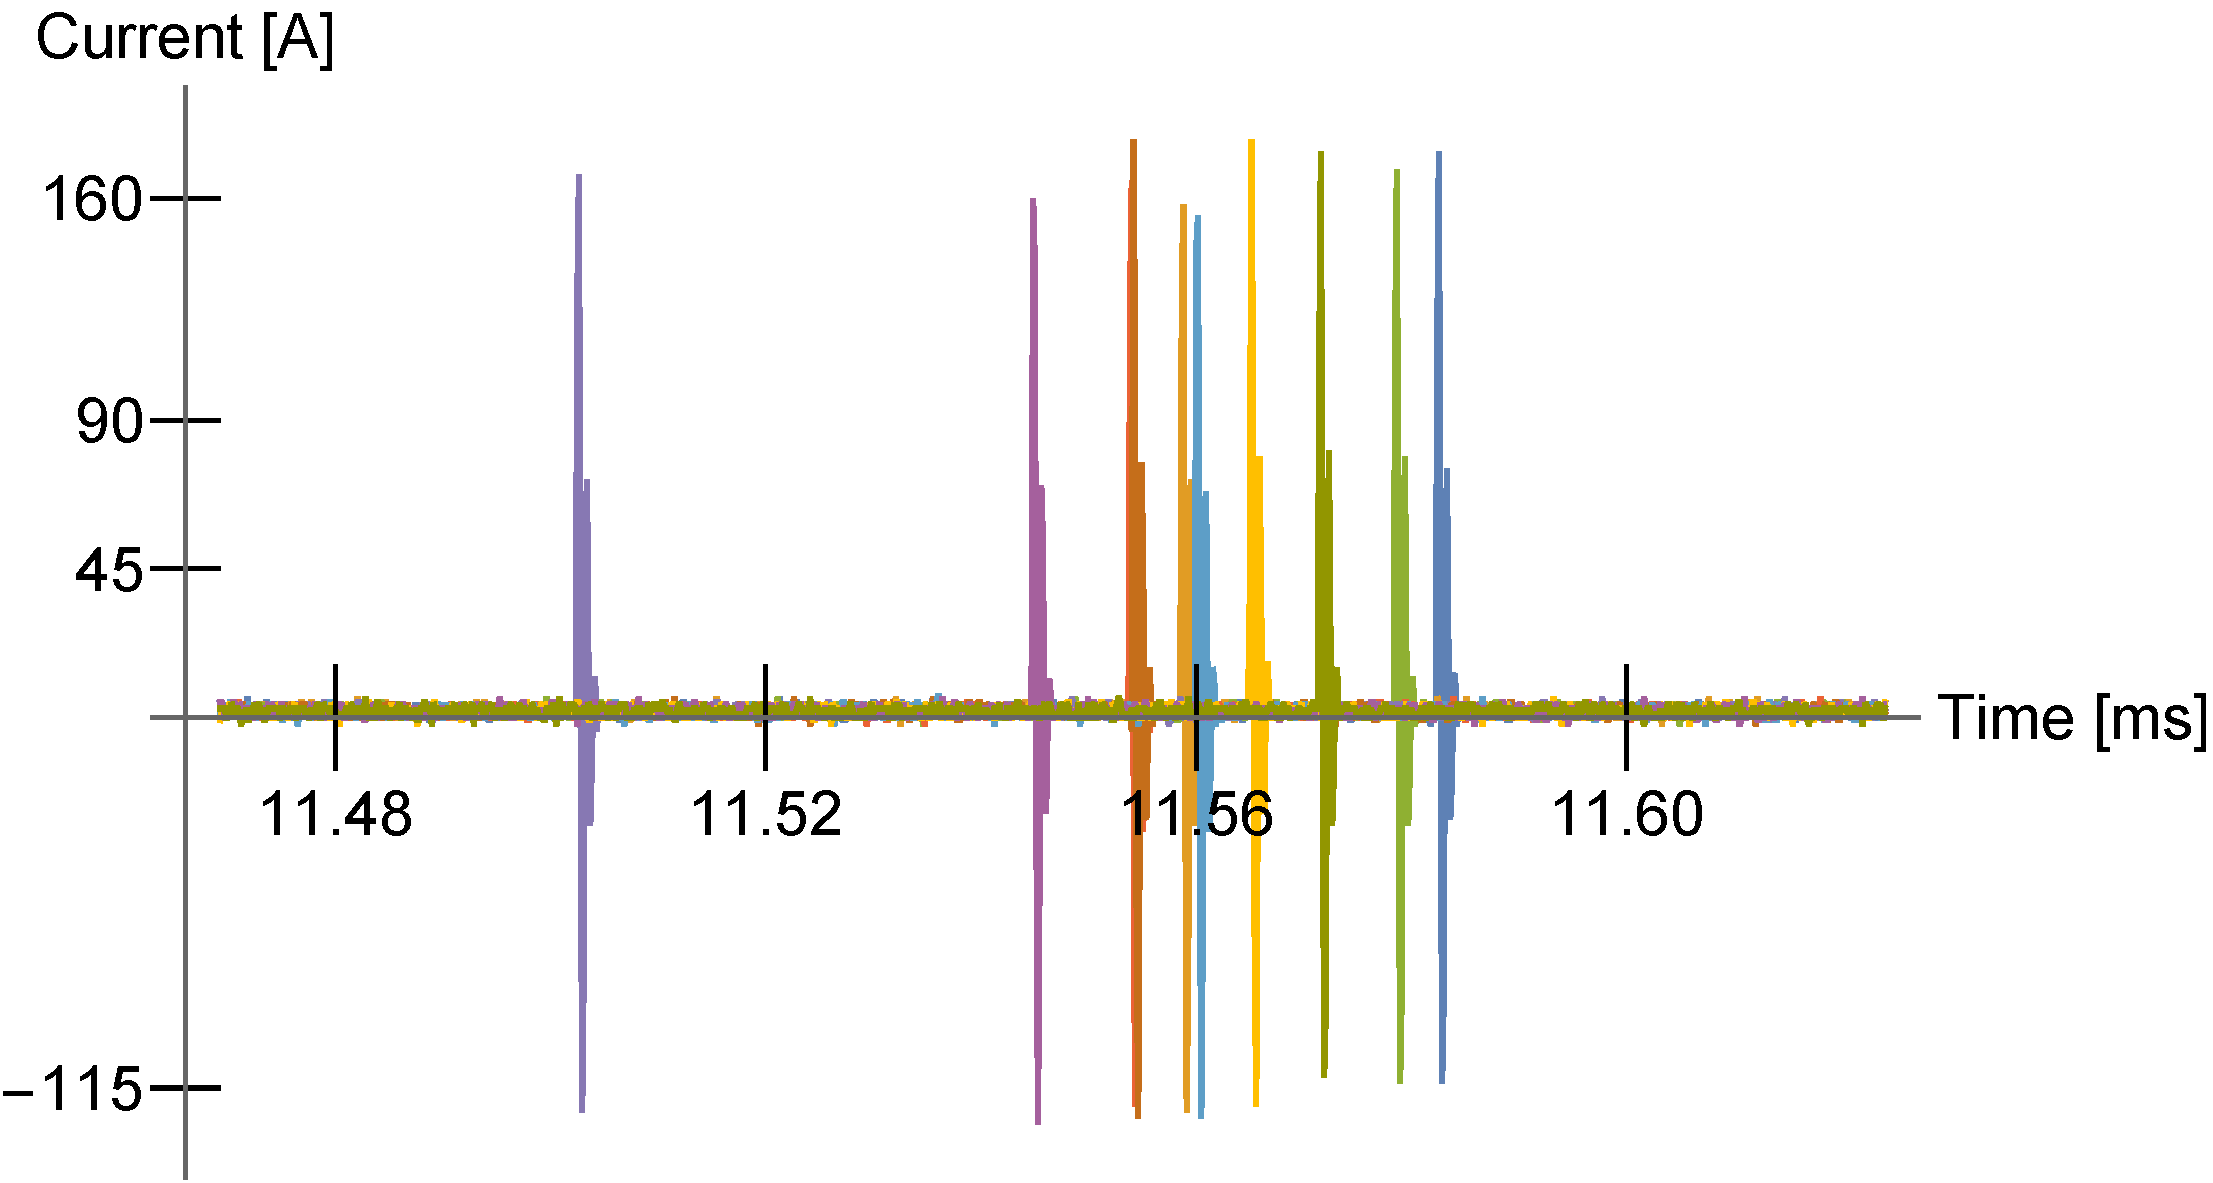
\includegraphics[width=\textwidth]{figures/jitter/multiple.pdf}
    \caption{Exposition of high jitter in the discharge when no Nd:Yag is present. \textcolor{red}{write this again.}}
    \label{fig:multiple}
\end{figure}

\section{Duration of the hollow density profile}\label{sec:duration-of-guiding}
We are now in a position to estimate the timing and duration of the hollow density profile. For that, with the system set--up as in the previous measurement, we aligned the \SI{800}{\nm} oscillator laser (\ref{ssec:lasers}) through the capillary and directed the outgoing beam out of the vacuum chamber to the active area of a fast photo-diode detector. This detector output was connected to the same measuring oscilloscope as well.

\begin{figure}
\centering 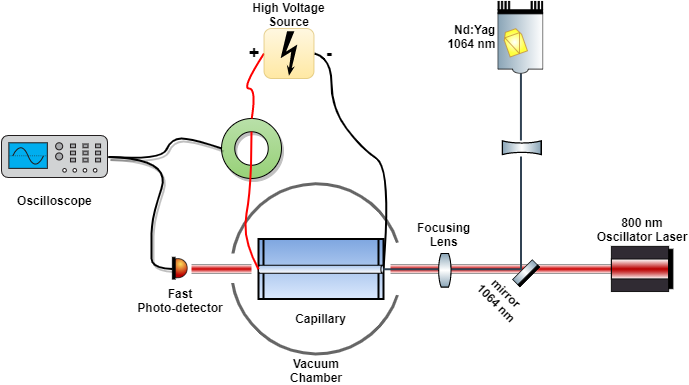
\includegraphics[width=\textwidth]{figures/oscillator.png}
\caption{\textcolor{red}{write a description.}}
\label{fig:oscillator}
\end{figure}
Upon plasma discharge, we recorded the optical guiding of the \textcolor{red}{ultra-}short laser pulses, shown in figure  \ref{fig:oscillator_single}, and watched after the gain of the signal while it interacts with the plasma inside the capillary. The result is shown in figure \ref{fig:oscillator_gain}.

The \textcolor{red}{color1} waveform is the plasma discharge current profile delivered from the Rogowsky coil. The \textcolor{red}{color2} waveform is the signal arriving from the Nd:Yag photo-diode detector, which as mentioned before, tells us whether the discharge is timed with the igniting laser and is jitter-controlled. The bottom, \textcolor{red}{color3} waveform is that recorded from \textcolor{red}{P.D 2} with the oscillator as its signal.
\begin{figure}
    \centering
    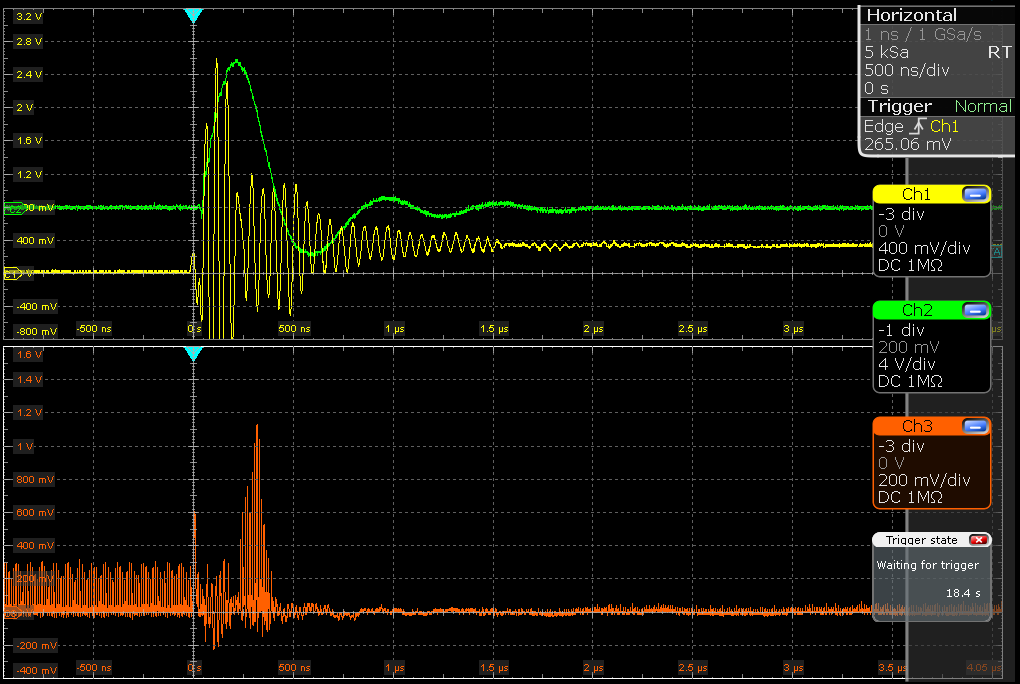
\includegraphics[width=\textwidth]{figures/gain.PNG}
    \caption{\textcolor{red}{Write.}}
    \label{fig:oscillator_gain}
\end{figure}

The explanation for the gain of the voltage arriving from \textcolor{red}{P.D 2} during the formation of the plasma channel was mentioned in section \ref{sec:indexrefraction}: If the plasma has a normal density profile (maximum on the axis), it behaves like a negative lens and causes the laser beam to diverge into the walls. If an inverted density profile (minimum on the axis, refer to figure \ref{fig:rdp_parabola}) can be created, however, the lens effect becomes converging; and the radiation is focused and trapped by the plasma. See figure \ref{fig:chen4_31}.
\begin{marginfigure}
		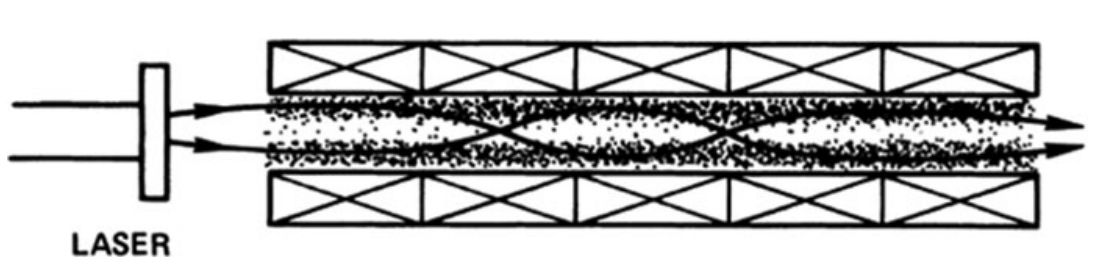
\includegraphics[width=\marginparwidth]{./figures/chen4_31.PNG}
		\caption{A plasma confined inside the capillary will trap the \SI{800}{\nm} laser light only if the plasma has a density minimum on axis.}
		\label{fig:chen4_31}
\end{marginfigure}

An additional phenomenon to remark is the attenuation of the signal in the later stage of the discharge---the plasma becomes opaque to radiation traversing it. \textcolor{red}{\textbf{Explain why}}

In addition to the timing and duration of the plasma channel, we examined the factor within which the guidance efficiency is determined. Therefore, we measured the enhancement for different parameters: applied voltage, laser power and injected gas pressure. Analysis shows that the main parameter that increases the efficiency of the guiding is the applied voltage. The effect is easily visible--the enhanced transmission duration is approximately in the scale of several \SI{1e-7}{\sec}, also we see that the timing seems to be synchronized with the maximal value of the current. Furthermore, using more precise analysis we assess the mean duration of the hollow density profile to be $\tau_\text{channel}=\SI{300}{\ns}$ and with a maximal transmission lasting approximately \SI{30}{\ns} long.

\section{Spectroscopic measurements}\label{sec:spectro}
To estimate \textcolor{red}{quantitatively} the depth of the plasma channel and the plasma density, we performed an additional measurement with a spectrometer and a fast camera, introduced in section \ref{ssec:spectro}, and analysed the broadened emission line attributable to Stark effect.

\subsection{Radial density profile}\label{ssec:radial}
We installed an imaging system that images the \textcolor{red}{spatially} capillary entrance, shown in figure \ref{fig:radial_system}. For an accurate and \textcolor{red}{fidelity?} measurement, we needed to over--come two main difficulties:

	\begin{figure}
	\centering
	    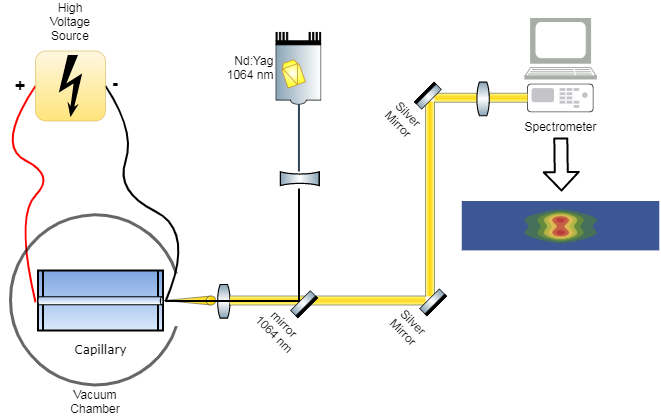
\includegraphics[width=\textwidth]{./figures/spectro/radial_system.png}
	    \caption{Experimental setup and typical spectrum of the plasma at the exit of the capillary.}
	    \label{fig:radial_system}
	\end{figure}

In order to magnify the circular cone of plasma light emitted from the capillary entrance imaged on the spectrometer slit, we placed a converging lens in a distance a bit longer from its focal length so to obtain as large as possible transverse magnification. The drawback is the loss of irradiance, which was compensated with the gain mechanism of the microchannel plate of the CCD camera.

Secondly, as mentioned before (\ref{sec:jitter}), the plasma channel lasts for \SIrange{50}{100}{\ns}, and this leads to a constraint on the duration of the camera gating window. Clearly, a long exposure time ($\gtrsim \SI{1}{\us}$) would yield a constant profile. But to capture the hollow plasma channel we rather gated (using the digital delay generator) the CCD camera to exposure times of \SI{40}{\ns}\marginnote{To produce a sharp image of a moving subject, a fast shutter speed is required.}. That obviously led to signal--to--noise--ratio difficulties when analysing the digital data --- the shutter is not opened for long enough for the image-sensing area to be exposed to light.

The simple imaging system was composed of two converging lens (fused-silica, bi-convex, \diameter 2 inch), the first with a shorter focal length, that imaged the capillary entrance magnified by $\times 5$ on the spectrometer entrance slit. I.e. the image of a \SI{0.5}{\mm} capillary was $\sim$ \SI{2.5}{\mm} in diameter, corresponding to about \textcolor{red}{???} of the CCD's vertical range. The spectrometer slit had the width of \SI{150}{\micro\metre}, providing a spectral resolution of about \SI{0.3}{\nm}.

The grating was rotated to the central wavelength of \SI{653.3}{\nm}, which, as mentioned in section \ref{sec:hydrogen}, is the unperturbed central wavelength of hydrogen H\textsubscript{$\alpha$} line. This line, when emitted within a plasma, undergoes Stark broadening from which the electron density can be deduced, with the density estimate based on equation \ref{eq:delta_lambda}. A dielectric mirror coated for zero degrees at \SI{1.064}{\um} prevented the radiation of the igniting laser from entering the spectrometer.

We gated the CCD camera, as stated, to \SI{40}{\ns} gate--on time at time windows that correspond to the maximal transmission of the oscillator signal (as described in \ref{sec:duration-of-guiding}), and set the gain of the microchannel plate to its highest, at the level of 9.

The raw spectroscopic images captured by \textit{Andor} in a \texttt{.fit} file format were processed in the \textit{Matlab} environment and its curve-fitting tool. A Lorentzian intensity profile is assumed as the analytical fitting function with the line half-width as a free parameter. A fit was found for each row of the data. The vertical dimension corresponds to the spatial coordinate. \textcolor{red}{Explain the step--by--step of the analysis or not?.}

Figure \ref{fig:plasma_channel_spectro} plots the experimentally measured plasma density as a function of position (capillary radius) across a \SI{500}{\um} capillary diameter at a delay time \SI{400}{\ns}\textcolor{red}{check the time} after the beginning of the electrical current. The maximum discharge current was \SI{160}{\A} \textcolor{red}{check the amperes}.

\begin{figure}
\centering
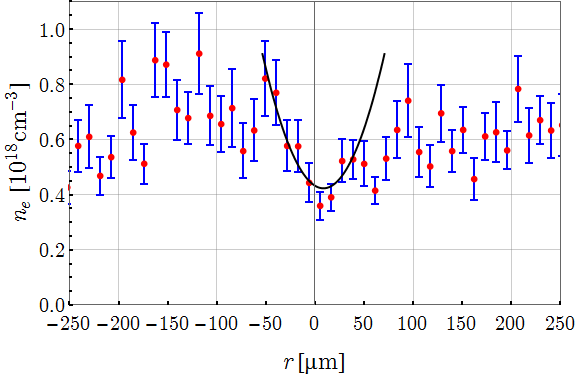
\includegraphics[width=\textwidth]{figures/spectro/parabolic.png}
    \caption{Radial density profile of the plasma from the measured spectrum, \SI{400}{\ns} \textcolor{red}{check the number} after the beginning of the current.}
    
\label{fig:plasma_channel_spectro}
\end{figure}

For these conditions, there is a density minimum on the axis of the capillary; at early delay times the minimum at the radial density profile was not created, and at later delay times it disappears. These conditions provide an optimal plasma channel that can be used for guiding an intense laser pulse for LWFA accelerators.

\subsection{Longitudinal density profile}\label{ssec:longi}

The method described in section \ref{ssec:radial} allows for measuring the radial density profile only at the capillary output. It is also important to verify longitudinal homogeneity of the plasma density. For this measurement the entire length of the \SI{5}{\cm} capillary was imaged along the entrance slit of the spectrometer.

To achieve that, we built the system shown in figure \ref{fig:longi_system}, with the main difference from the one before, figure \ref{fig:radial_system}, being the periscope assembly used to rotate the stripe of plasma emission by \SI{90}{\degree} so it can enters into the entrance slit of the spectrometer. As opposed to the magnification issue we had before, now a minification of the image was sought. We positioned the capillary on a moveable mount, and made a 


from this \href{article}{https://aip.scitation.org/doi/pdf/10.1063/1.5046400}: avalanche ablative process is started, and due to the discharge current, a plasma is formed in the capillaries.

See this \href{https://tex.stackexchange.com/a/427625}{Answer} to integrating draw.io with LaTeX.
Mathematica customizing error bars answer:
mathematica.stackexchange id 210185
https://mathematica.stackexchange.com/questions/210185/customising-error-bars-in-mathematica-12
\printbibliography

\end{document}
